\documentclass{beamer}

\usepackage{fontawesome}
\usepackage[backend=bibtex]{biblatex}
\usepackage[T1]{fontenc}

\addbibresource{sources.bib}

\graphicspath{ {../images}}  % assumes it is being built in presentation/build dir

\makeatletter
\newenvironment{myitemize}{%
   \setlength{\topsep}{0pt}
   \setlength{\partopsep}{0pt}
   \renewcommand*{\@listi}{\leftmargin\leftmargini \parsep\z@ \topsep\z@ \itemsep\z@}
   \let\@listI\@listi
   \itemize
}{\enditemize}
\makeatother  

%Information to be included in the title page:
\title{Dynamiczna alokacja pamięci w embedded}
\author{Paweł Warzecha}
\institute{Wro.cpp}
\date{07.05.2025}

\begin{document}

\frame{\titlepage}
%%%%%%%%%%%%%%%%%%%%%%%%%%%%%%%%%%%%%%%%%%%%%%%%%%%%%%%%%%%%%%%%%%%%%%%%
\begin{frame}[t]
    \frametitle{Dlaczego nie używać dynamicznej alokacji}
\end{frame}
%%%%%%%%%%%%%%%%%%%%%%%%%%%%%%%%%%%%%%%%%%%%%%%%%%%%%%%%%%%%%%%%%%%%%%%%
\begin{frame}[t]
    \frametitle{Dlaczego nie używać dynamicznej alokacji}
    \begin{columns}[t]
        \begin{column}[t]{0.35\textwidth}
            \begin{myitemize}
                \item Nie da się
            \end{myitemize}
        \end{column}
        \begin{column}[t]{0.7\textwidth}
        \end{column}
    \end{columns}
\end{frame}
%%%%%%%%%%%%%%%%%%%%%%%%%%%%%%%%%%%%%%%%%%%%%%%%%%%%%%%%%%%%%%%%%%%%%%%%
\begin{frame}[t]
    \frametitle{Dlaczego nie używać dynamicznej alokacji}
    \begin{columns}[t]
        \begin{column}[t]{0.35\textwidth}
            \begin{myitemize}
                \item Nie da się
            \end{myitemize}
        \end{column}
        \begin{column}[t]{0.7\textwidth}
            \begin{center}
            \includegraphics[width=0.9\textwidth]{reddit}\\
            \tiny \cite{reddit} 
            \end{center}
        \end{column}
    \end{columns}
\end{frame}
%%%%%%%%%%%%%%%%%%%%%%%%%%%%%%%%%%%%%%%%%%%%%%%%%%%%%%%%%%%%%%%%%%%%%%%%
\begin{frame}[t]
    \frametitle{Dlaczego nie używać dynamicznej alokacji}

    \begin{columns}
        \begin{column}[t]{0.35\textwidth}
            \begin{myitemize}
                \item Nie da się
                \item Mało pamięci
            \end{myitemize}
        \end{column}
        \begin{column}[t]{0.7\textwidth}
            \begin{center}
            \includegraphics[width=0.9\textwidth]{reddit}\\
            \tiny \cite{reddit} 
            \end{center}
        \end{column}
    \end{columns}
\end{frame}
%%%%%%%%%%%%%%%%%%%%%%%%%%%%%%%%%%%%%%%%%%%%%%%%%%%%%%%%%%%%%%%%%%%%%%%%
\begin{frame}[t]
    \frametitle{Dlaczego nie używać dynamicznej alokacji}

    \begin{columns}[t]
        \begin{column}[t]{0.35\textwidth}
            \begin{myitemize}
                \item Nie da się
                \item Mało pamięci
                \item Niezawodność
            \end{myitemize}
        \end{column}
        \begin{column}[t]{0.7\textwidth}
            \begin{center}
                \includegraphics[width=0.9\textwidth]{reddit}\\
                \tiny \cite{reddit} 
            \end{center}
        \end{column}
    \end{columns}
\end{frame}
%%%%%%%%%%%%%%%%%%%%%%%%%%%%%%%%%%%%%%%%%%%%%%%%%%%%%%%%%%%%%%%%%%%%%%%%
\begin{frame}[t]
    \frametitle{Dlaczego nie używać dynamicznej alokacji}

    \begin{columns}[t]
        \begin{column}[t]{0.35\textwidth}
            \begin{myitemize}
                \item Nie da się
                \item Mało pamięci
                \item Niezawodność
            \end{myitemize}
        \end{column}
        \begin{column}[t]{0.7\textwidth}
            \begin{center}
                \includegraphics[width=0.9\textwidth]{stackoverflow}\\
                \tiny \cite{stackoverflow} 
            \end{center}
        \end{column}
    \end{columns}
\end{frame}
%%%%%%%%%%%%%%%%%%%%%%%%%%%%%%%%%%%%%%%%%%%%%%%%%%%%%%%%%%%%%%%%%%%%%%%%
\begin{frame}[t]
    \frametitle{Dlaczego nie używać dynamicznej alokacji}

    \begin{columns}[t]
        \begin{column}[t]{0.35\textwidth}
            \begin{myitemize}
                \item Nie da się
                \item Mało pamięci
                \item Niezawodność
                \item Fragmentacja
            \end{myitemize}
        \end{column}
        \begin{column}[t]{0.7\textwidth}
            \begin{center}
                \includegraphics[width=0.9\textwidth]{stackoverflow}\\
                \tiny \cite{stackoverflow} 
            \end{center}
        \end{column}
    \end{columns}
\end{frame}
%%%%%%%%%%%%%%%%%%%%%%%%%%%%%%%%%%%%%%%%%%%%%%%%%%%%%%%%%%%%%%%%%%%%%%%%
\begin{frame}[t]
    \frametitle{Dlaczego nie używać dynamicznej alokacji}

    \begin{columns}[t]
        \begin{column}[t]{0.35\textwidth}
            \begin{myitemize}
                \item Nie da się
                \item Mało pamięci
                \item Niezawodność
                \item Fragmentacja
                \item Szybkość
            \end{myitemize}
        \end{column}
        \begin{column}[t]{0.7\textwidth}
            \begin{center}
                \includegraphics[width=0.9\textwidth]{stackoverflow}\\
                \tiny \cite{stackoverflow} 
            \end{center}
        \end{column}
    \end{columns}
\end{frame}
%%%%%%%%%%%%%%%%%%%%%%%%%%%%%%%%%%%%%%%%%%%%%%%%%%%%%%%%%%%%%%%%%%%%%%%%
\begin{frame}[t]
    \frametitle{Dlaczego nie używać dynamicznej alokacji}

    \begin{columns}[t]
        \begin{column}[t]{0.35\textwidth}
            \begin{myitemize}
                \item Nie da się
                \item Mało pamięci
                \item Niezawodność
                \item Fragmentacja
                \item Szybkość
            \end{myitemize}
        \end{column}
        \begin{column}[t]{0.7\textwidth}
            \begin{center}
                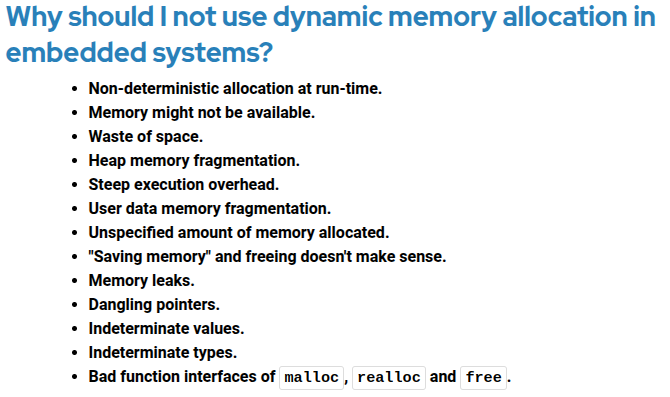
\includegraphics[width=0.9\textwidth]{codidact}\\
                \tiny \cite{codidact} 
            \end{center}
        \end{column}
    \end{columns}
\end{frame}
%%%%%%%%%%%%%%%%%%%%%%%%%%%%%%%%%%%%%%%%%%%%%%%%%%%%%%%%%%%%%%%%%%%%%%%%
\begin{frame}
    \frametitle{Nie da się}
    \begin{center}
        \includegraphics[width=0.9\textwidth]{just_new}
    \end{center}
\end{frame}
%%%%%%%%%%%%%%%%%%%%%%%%%%%%%%%%%%%%%%%%%%%%%%%%%%%%%%%%%%%%%%%%%%%%%%%%
\begin{frame}[t]
    \frametitle{Mało pamięci}
    \begin{columns}[t]
        \begin{column}{0.5\textwidth}
            \begin{center}
                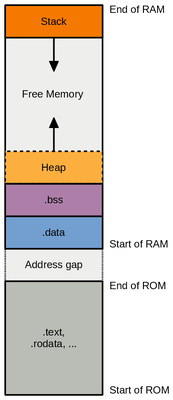
\includegraphics[height=0.6\textheight]{memory}\\
                \tiny \cite{memory} 
            \end{center}
        \end{column}
        \begin{column}[t]{0.5\textwidth}
        \end{column}
    \end{columns}
\end{frame}
%%%%%%%%%%%%%%%%%%%%%%%%%%%%%%%%%%%%%%%%%%%%%%%%%%%%%%%%%%%%%%%%%%%%%%%%
\begin{frame}[t]
    \frametitle{Mało pamięci}
    \begin{columns}[t]
        \begin{column}{0.5\textwidth}
            \begin{center}
                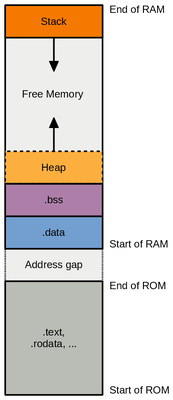
\includegraphics[height=0.6\textheight]{memory}\\
                \tiny \cite{memory} 
            \end{center}
        \end{column}
        \begin{column}[t]{0.5\textwidth}
            \begin{center}
                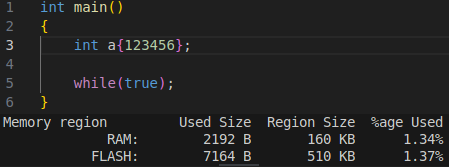
\includegraphics[width=0.75\textwidth]{singel_stack_variable_memory}
            \end{center}
        \end{column}
    \end{columns}
\end{frame}
%%%%%%%%%%%%%%%%%%%%%%%%%%%%%%%%%%%%%%%%%%%%%%%%%%%%%%%%%%%%%%%%%%%%%%%%
\begin{frame}[t]
    \frametitle{Mało pamięci}
    \begin{columns}[t]
        \begin{column}{0.5\textwidth}
            \begin{center}
                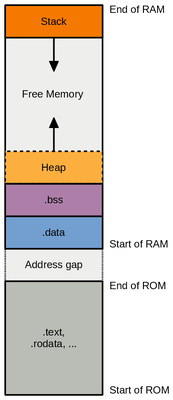
\includegraphics[height=0.6\textheight]{memory}\\
                \tiny \cite{memory} 
            \end{center}
        \end{column}
        \begin{column}[t]{0.5\textwidth}
            \begin{center}
                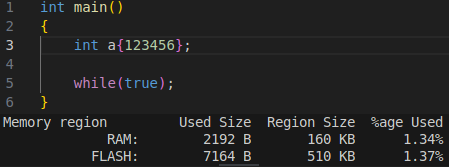
\includegraphics[width=0.75\textwidth]{singel_stack_variable_memory}

                \vspace{5 mm}

                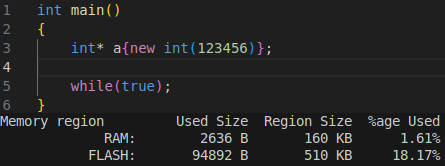
\includegraphics[width=0.75\textwidth]{just_new_memory}
            \end{center}
        \end{column}
    \end{columns}
\end{frame}
%%%%%%%%%%%%%%%%%%%%%%%%%%%%%%%%%%%%%%%%%%%%%%%%%%%%%%%%%%%%%%%%%%%%%%%%
\begin{frame}[t]
    \frametitle{Mało pamięci}
    \begin{columns}[t]
        \begin{column}{0.5\textwidth}
            \begin{center}
                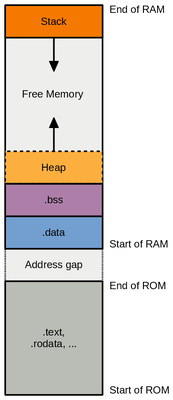
\includegraphics[height=0.6\textheight]{memory}\\
                \tiny \cite{memory} 
            \end{center}
        \end{column}
        \begin{column}[t]{0.5\textwidth}
            \begin{center}
                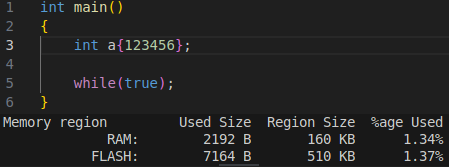
\includegraphics[width=0.75\textwidth]{singel_stack_variable_memory}

                \vspace{5 mm}

                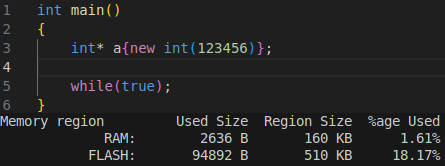
\includegraphics[width=0.75\textwidth]{just_new_memory}

                \vspace{5 mm}

                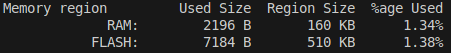
\includegraphics[width=0.75\textwidth]{just_new_memory_o2}
            \end{center}
        \end{column}
    \end{columns}
\end{frame}
%%%%%%%%%%%%%%%%%%%%%%%%%%%%%%%%%%%%%%%%%%%%%%%%%%%%%%%%%%%%%%%%%%%%%%%%
\begin{frame}[t]
    \frametitle{Mało pamięci}
    \begin{columns}[t]
        \begin{column}{0.5\textwidth}
            \begin{center}
                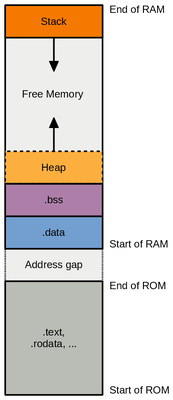
\includegraphics[height=0.6\textheight]{memory}\\
                \tiny \cite{memory} 
            \end{center}
        \end{column}
        \begin{column}[t]{0.5\textwidth}
            \begin{center}
                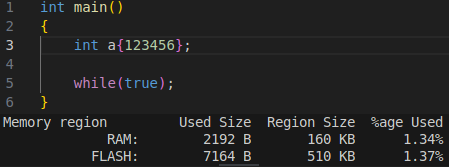
\includegraphics[width=0.75\textwidth]{singel_stack_variable_memory}

                \vspace{5 mm}

                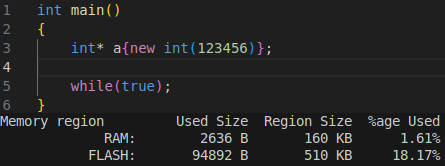
\includegraphics[width=0.75\textwidth]{just_new_memory}

                \vspace{5 mm}

                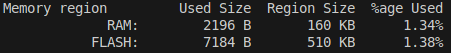
\includegraphics[width=0.75\textwidth]{just_new_memory_o2}
            \end{center}
        \end{column}
    \end{columns}
    \begin{center}
        \includegraphics[width=0.6\textwidth]{allocation}
        \tiny \cite{allocation} 
    \end{center}
\end{frame}
%%%%%%%%%%%%%%%%%%%%%%%%%%%%%%%%%%%%%%%%%%%%%%%%%%%%%%%%%%%%%%%%%%%%%%%%
\begin{frame}[t]
    \frametitle{Szybkość}
    \begin{columns}[t]
        \begin{column}[t]{0.5\textwidth}
            \begin{center}
                \includegraphics[height=0.5\textheight]{stack_alocation_time}
            \end{center}
        \end{column}
        \begin{column}[t]{0.5\textwidth}
        \end{column}
    \end{columns}
\end{frame}
%%%%%%%%%%%%%%%%%%%%%%%%%%%%%%%%%%%%%%%%%%%%%%%%%%%%%%%%%%%%%%%%%%%%%%%%
\begin{frame}[t]
    \frametitle{Szybkość}
    \begin{columns}[t]
        \begin{column}[t]{0.5\textwidth}
            \begin{center}
                \includegraphics[height=0.5\textheight]{stack_alocation_time}
            \end{center}
        \end{column}
        \begin{column}[t]{0.5\textwidth}
            \begin{center}
                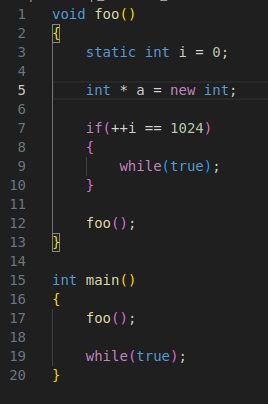
\includegraphics[height=0.5\textheight]{heap_allocation_time}
            \end{center}
        \end{column}
    \end{columns}
\end{frame}
%%%%%%%%%%%%%%%%%%%%%%%%%%%%%%%%%%%%%%%%%%%%%%%%%%%%%%%%%%%%%%%%%%%%%%%%
\begin{frame}[t]
    \frametitle{Szybkość}
    \begin{columns}[t]
        \begin{column}[t]{0.5\textwidth}
            \begin{center}
                \includegraphics[height=0.5\textheight]{stack_alocation_time}
            \end{center}
        \end{column}
        \begin{column}[t]{0.5\textwidth}
            \begin{center}
                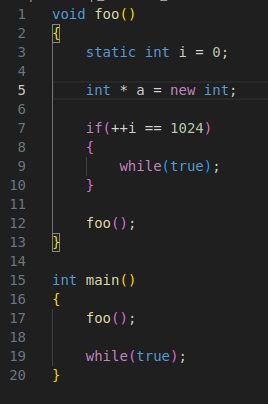
\includegraphics[height=0.5\textheight]{heap_allocation_time}
            \end{center}
        \end{column}
    \end{columns}
    \begin{center}
        \begin{tabular}{|| r | c | c | c ||}
        \hline
         & Total [clock cycles] & Jedna iteracja & Diff to baseline \\ [0.2ex] 
        \hline
        \hline
        baseline & 32765 & 32 & - \\
        \hline
        \end{tabular}
    \end{center}
\end{frame}
%%%%%%%%%%%%%%%%%%%%%%%%%%%%%%%%%%%%%%%%%%%%%%%%%%%%%%%%%%%%%%%%%%%%%%%%
\begin{frame}[t]
    \frametitle{Szybkość}
    \begin{columns}[t]
        \begin{column}[t]{0.5\textwidth}
            \begin{center}
                \includegraphics[height=0.5\textheight]{stack_alocation_time}
            \end{center}
        \end{column}
        \begin{column}[t]{0.5\textwidth}
            \begin{center}
                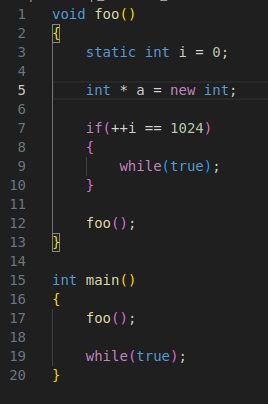
\includegraphics[height=0.5\textheight]{heap_allocation_time}
            \end{center}
        \end{column}
    \end{columns}
    \begin{center}
        \begin{tabular}{|| r | c | c | c ||}
        \hline
         & Total [clock cycles] & Jedna iteracja & Diff to baseline \\ [0.2ex] 
        \hline
        \hline
        baseline & 32765 & 32 & - \\
        \hline
        stack & 33789 & 33 & 1 \\
        \hline
        \end{tabular}
    \end{center}
\end{frame}
%%%%%%%%%%%%%%%%%%%%%%%%%%%%%%%%%%%%%%%%%%%%%%%%%%%%%%%%%%%%%%%%%%%%%%%%
\begin{frame}[t]
    \frametitle{Szybkość}
    \begin{columns}[t]
        \begin{column}[t]{0.5\textwidth}
            \begin{center}
                \includegraphics[height=0.5\textheight]{stack_alocation_time}
            \end{center}
        \end{column}
        \begin{column}[t]{0.5\textwidth}
            \begin{center}
                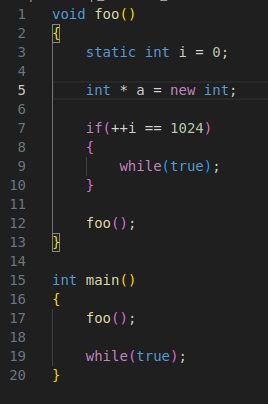
\includegraphics[height=0.5\textheight]{heap_allocation_time}
            \end{center}
        \end{column}
    \end{columns}
    \begin{center}
        \begin{tabular}{|| r | c | c | c ||}
        \hline
         & Total [clock cycles] & Jedna iteracja & Diff to baseline \\ [0.2ex] 
        \hline
        \hline
        baseline & 32765 & 32 & - \\
        \hline
        stack & 33789 & 33 & 1 \\
        \hline
        heap & 141781 & 138 & 106 \\
        \hline
        \end{tabular}
    \end{center}
\end{frame}
%%%%%%%%%%%%%%%%%%%%%%%%%%%%%%%%%%%%%%%%%%%%%%%%%%%%%%%%%%%%%%%%%%%%%%%%
\begin{frame}[t]
    \frametitle{Fragmentacja}

    \begin{center}
        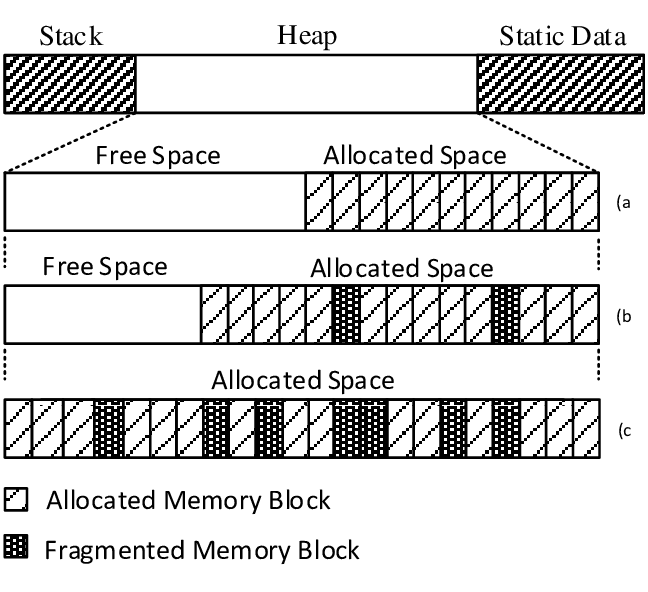
\includegraphics[width=0.5\textwidth]{fragmentation}\\
        \tiny \cite{fragmentation} 
    \end{center}     
\end{frame}
%%%%%%%%%%%%%%%%%%%%%%%%%%%%%%%%%%%%%%%%%%%%%%%%%%%%%%%%%%%%%%%%%%%%%%%%
\begin{frame}[t]
    \frametitle{Fragmentacja}

    \begin{center}
        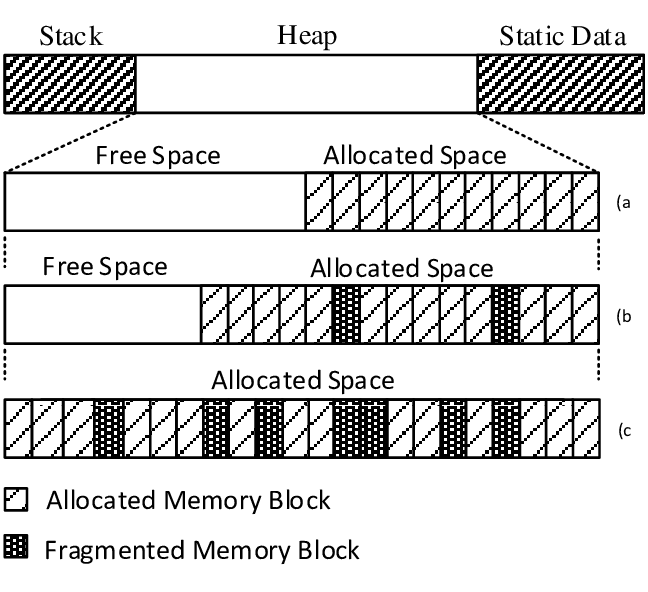
\includegraphics[width=0.5\textwidth]{fragmentation}\\
        \tiny \cite{fragmentation} \\

        \normalsize Alokacja na końcu: 145\\
    \end{center}     
\end{frame}
%%%%%%%%%%%%%%%%%%%%%%%%%%%%%%%%%%%%%%%%%%%%%%%%%%%%%%%%%%%%%%%%%%%%%%%%
\begin{frame}[t]
    \frametitle{Fragmentacja}

    \begin{center}
        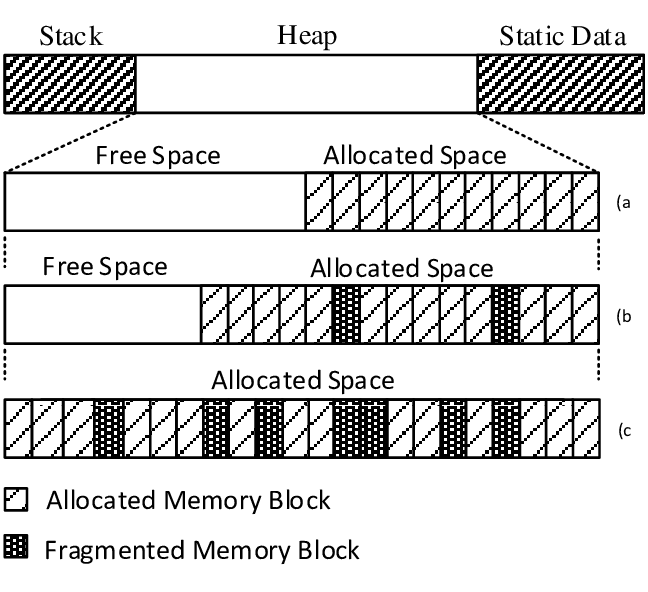
\includegraphics[width=0.5\textwidth]{fragmentation}\\
        \tiny \cite{fragmentation} \\

        \normalsize Alokacja na końcu: 145\\
        \normalsize Alokacja w pofragmentowanej pamięci: 264
    \end{center}     
\end{frame}
%%%%%%%%%%%%%%%%%%%%%%%%%%%%%%%%%%%%%%%%%%%%%%%%%%%%%%%%%%%%%%%%%%%%%%%%
\begin{frame}[t]
    \frametitle{Niezawodność}

    \begin{center}
        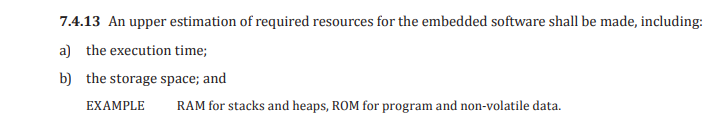
\includegraphics[width=0.5\textwidth]{iso26262}\\
        \tiny \cite{iso26262} ISO-26262\\
    \end{center}     
\end{frame}
%%%%%%%%%%%%%%%%%%%%%%%%%%%%%%%%%%%%%%%%%%%%%%%%%%%%%%%%%%%%%%%%%%%%%%%%
\begin{frame}[t]
    \frametitle{Niezawodność}

    \begin{center}
        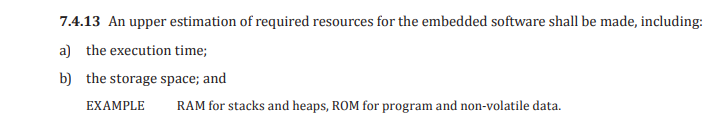
\includegraphics[width=0.5\textwidth]{iso26262}\\
        \tiny \cite{iso26262} ISO-26262\\
        \vspace{5 mm}
        \includegraphics[width=0.5\textwidth]{DO-178C}\\
        \tiny \cite{do178c} DO-178C\\        
    \end{center}     
\end{frame}
%%%%%%%%%%%%%%%%%%%%%%%%%%%%%%%%%%%%%%%%%%%%%%%%%%%%%%%%%%%%%%%%%%%%%%%%
\begin{frame}[t]
    \frametitle{Niezawodność}

    \begin{center}
        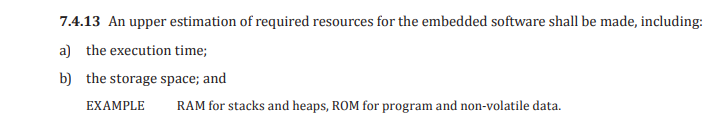
\includegraphics[width=0.5\textwidth]{iso26262}\\
        \tiny \cite{iso26262} ISO-26262\\
        \vspace{5 mm}
        \includegraphics[width=0.5\textwidth]{DO-178C}\\
        \tiny \cite{do178c} DO-178C\\      
        \vspace{5 mm}
        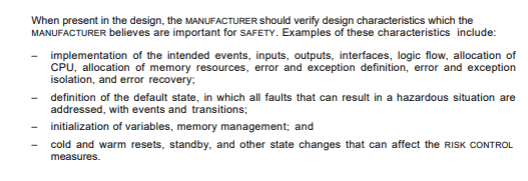
\includegraphics[width=0.5\textwidth]{iec62304}\\
        \tiny \cite{iec62304} IEC-62304\\          
    \end{center}     
\end{frame}
%%%%%%%%%%%%%%%%%%%%%%%%%%%%%%%%%%%%%%%%%%%%%%%%%%%%%%%%%%%%%%%%%%%%%%%%
\begin{frame}[t]
    \frametitle{Niezawodność}

    \begin{center}
        \includegraphics[width=0.5\textwidth]{misrac++2008}\\
        \tiny \cite{misrac++2008} misra c++ 2008\\
    \end{center}    
\end{frame}
%%%%%%%%%%%%%%%%%%%%%%%%%%%%%%%%%%%%%%%%%%%%%%%%%%%%%%%%%%%%%%%%%%%%%%%%
\begin{frame}[t]
    \frametitle{Niezawodność}

    \begin{center}
        \includegraphics[width=0.5\textwidth]{misrac++2008}\\
        \tiny \cite{misrac++2008} misra c++ 2008\\
        \vspace{5 mm}
        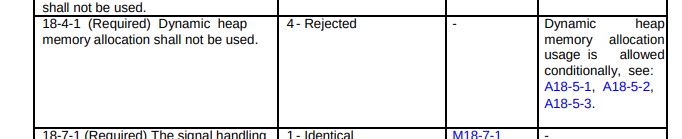
\includegraphics[width=0.5\textwidth]{autosarc++}\\
        \tiny \cite{autosarc++14} autosar c++14 guidelines\\  
    \end{center}    
\end{frame}
%%%%%%%%%%%%%%%%%%%%%%%%%%%%%%%%%%%%%%%%%%%%%%%%%%%%%%%%%%%%%%%%%%%%%%%%
\begin{frame}[t]
    \frametitle{Niezawodność}

    \begin{center}
        \includegraphics[width=0.5\textwidth]{misrac++2008}\\
        \tiny \cite{misrac++2008} misra c++ 2008\\
        \vspace{5 mm}
        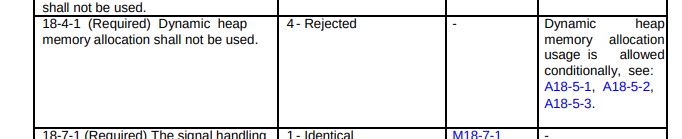
\includegraphics[width=0.5\textwidth]{autosarc++}\\
        \tiny \cite{autosarc++14} autosar c++14 guidelines\\  
        \vspace{5 mm}
        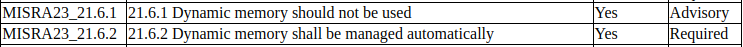
\includegraphics[width=0.5\textwidth]{misra23}\\
        \tiny \cite{misrac++2023} misra c++ 2023\\  
    \end{center}    
\end{frame}
%%%%%%%%%%%%%%%%%%%%%%%%%%%%%%%%%%%%%%%%%%%%%%%%%%%%%%%%%%%%%%%%%%%%%%%%
\begin{frame}[t]
    \frametitle{Dlaczego nie używać dynamicznej alokacji}
    \begin{myitemize}
        \item Nie da się
    \end{myitemize}
\end{frame}
%%%%%%%%%%%%%%%%%%%%%%%%%%%%%%%%%%%%%%%%%%%%%%%%%%%%%%%%%%%%%%%%%%%%%%%%
\begin{frame}[t]
    \frametitle{Dlaczego nie używać dynamicznej alokacji}
    \begin{myitemize}
        \item Nie da się
        \item Mało pamięci
    \end{myitemize}
\end{frame}
%%%%%%%%%%%%%%%%%%%%%%%%%%%%%%%%%%%%%%%%%%%%%%%%%%%%%%%%%%%%%%%%%%%%%%%%
\begin{frame}[t]
    \frametitle{Dlaczego nie używać dynamicznej alokacji}
    \begin{myitemize}
        \item Nie da się
        \item Mało pamięci
        \item Szybkość
    \end{myitemize}
\end{frame}
%%%%%%%%%%%%%%%%%%%%%%%%%%%%%%%%%%%%%%%%%%%%%%%%%%%%%%%%%%%%%%%%%%%%%%%%
\begin{frame}[t]
    \frametitle{Dlaczego nie używać dynamicznej alokacji}
    \begin{myitemize}
        \item Nie da się
        \item Mało pamięci
        \item Szybkość
        \item Fragmentacja
    \end{myitemize}
\end{frame}
%%%%%%%%%%%%%%%%%%%%%%%%%%%%%%%%%%%%%%%%%%%%%%%%%%%%%%%%%%%%%%%%%%%%%%%%
\begin{frame}[t]
    \frametitle{Dlaczego nie używać dynamicznej alokacji}
    \begin{myitemize}
        \item Nie da się
        \item Mało pamięci
        \item Szybkość
        \item Fragmentacja
        \item Niezawodność
    \end{myitemize}
\end{frame}
%%%%%%%%%%%%%%%%%%%%%%%%%%%%%%%%%%%%%%%%%%%%%%%%%%%%%%%%%%%%%%%%%%%%%%%%
\begin{frame}
\begin{center}
    \vspace{20mm}
    \Huge Qustions?
\end{center}

\vspace{35mm}
\hspace{55mm}\tiny Paweł Warzecha\\
\hspace{55mm}\tiny \faGithub :  https://github.com/ProrokWielki\\
\hspace{55mm}\tiny \faLinkedin :  https://www.linkedin.com/in/pawel-warzecha/\\
\end{frame}
%%%%%%%%%%%%%%%%%%%%%%%%%%%%%%%%%%%%%%%%%%%%%%%%%%%%%%%%%%%%%%%%%%%%%%%%
\begin{frame}[t]
    All references:
    \AtNextBibliography{\tiny}
     \nocite{*}\printbibliography
\end{frame}

\end{document}